\section{Event Simulation}

The method by which all of the measurements presented in this thesis are performed is that of \emph{Monte-Carlo (MC) forward folding}. In a nutshell, this method involves producing a large set of simulated signal and background events that are then re-weighted in such a way that their distribution matches that of the observed data events as closely as possible. To give reliable results, an accurate simulation of all particle interactions described in Section~\ref{sec:particle-interactions} as well as the detector electronics described in section~\ref{sec:dom-daq} is required. The simulated and observed events are then passed through the same data processing chain described in section~\ref{sec:data-processing}. The resulting MC simulated dataset and the observed dataset are then histogrammed in the same binning, and the weights of the MC events are adjusted to give the best match between the histograms according to a loss function as defined in section~\ref{sec:test-statistic}.

The simulation chain for neutrinos and atmospheric muons can generally be divided into three steps that are described in this chapter:
\begin{enumerate}
    \item Simulation of particle interactions
    \item Photon propagation in ice
    \item Response of detector DAQ systems
\end{enumerate}
A special case is the simulation of detector noise, for which no particle production or photon propagation is necessary.

% \subsection{Particle Interactions}

% The first step for the simulation of neutrinos and muons is to sample parameters for the primary particle, and to simulate the secondary charged particles that are produced when it interacts inside the detector. The charged components of the secondary particles are then passed on to the photon propagation step described in section~\ref{sec:photon-propagation}.

\subsection{Neutrino Interactions}

Because of the inherently low interaction rate of neutrinos, it would be impractical to simulate a constant flux of neutrinos from any particular direction, the vast majority of which would simply pass through the detector without producing any signal at all. Instead, every simulated neutrino is forced to interact within a given volume, and the event is given a weight corresponding to the inverse of the simulated fluence,
\begin{equation}
    w = \frac{1}{F_{\mathrm{sim}}} \frac{1}{N_{\mathrm{sim}}}\;,
\end{equation}
where $N_{\mathrm{sim}}$ is the number of simulated events and $F_{\mathrm{sim}}$ is the fluence per area, solid angle, energy, and time. This weight, when multiplied with the flux of a given physics model and a live time, gives the expected number of events that this simulated event corresponds to.
\todo{Get feedback on whether it is necessary to explain in detail the sampling of the length traveled through the cylinder. As long as absorption is negligible, the given description should be simpler and exactly equivalent.}
%For this analysis, the simulated interaction volume is a cylinder centered in DeepCore, with a length and radius chosen such that all events that have a chance of producing a signal in DeepCore should be contained in it. The neutrino directions are sampled isotropically in azimuth and zenith, implying that the simulated flux per solid angle is $\phi_\Omega = \frac{1}{4\pi}$. The simulated neutrino flux is a power law with $\phi_e \propto E^{-2}$. After sampling the zenith and azimuth for an event, a random position is sampled  
Under the assumption that neutrino absorption is negligible and that the material consists of isoscalar targets, the simulated fluence is given by the chosen probability density in the direction and energy, $\phi_\Omega \times \phi_E$,  the size of the interaction volume, $V$, the cross-section of the interaction, $\sigma$, and the density of the material, $\rho$, by
\begin{equation}
    F_{\mathrm{sim}}^{-1} = V \times \rho \times N_A \times 1\frac{\mathrm{mol}}{\mathrm{g}} \times \sigma \times \frac{1}{\phi_\Omega} \times \frac{1}{\phi_E}\;,
\end{equation}
where $N_A$ is Avogadro's number. The volume in which neutrino interactions are simulated is a cylinder centered in DeepCore, with a length and radius chosen such that all events that have a chance of producing a signal in DeepCore should be contained in it, depending on the neutrino flavor and energy (see also table~\ref{table:GENIE}). Neutrino directions are isotropically distributed in zenith and azimuth, implying $\phi_\Omega = \frac{1}{4\pi}$. The neutrino energies are sampled from a power law with $\phi_e \propto E^{-2}$. The simulated live time corresponding to a single simulated event is  $T_{\mathrm{sim}} =  F_{\mathrm{sim}} / \Phi$, where $\Phi$ is the expected neutrino flux including neutrino oscillations at global best-fit parameters. The amount of simulation generated for each neutrino flavor is chosen such that the total simulated live time is $>70$~years over the entire energy range. Neutrinos and anti-neutrinos are produced in ratios of 70\% and 30\%, respectively. The simulated live time as a function of energy is shown in figure~\ref{fig:sim-livetime}. The livetime for electron neutrinos is increasing with energy because the simulated spectrum is harder than the real spectrum. The livetime for tau neutrinos is much higher than that of other flavors because the contribution of tau neutrinos to the expected neutrino flux is very small.

\begin{table}
\caption{Table of generation volumes used for \textsc{Genie} neutrino simulation. The cylinder is centered in DeepCore in all cases. \label{table:GENIE}}
\begin{center}
\begin{tabular}{ ccccc } 
\textbf{Flavor} & \textbf{Energy (GeV)} & \textbf{Radius (m)} & \textbf{Length (m)}\\
\toprule
\multirow{4}{*}{$\nu_e+\bar{\nu_e}$}  & 1-4 & 250 & 500 \\
 & 4-12 & 250 & 500   \\ 
 & 12-100 & 350 & 600  \\
 & 100-10000 & 550 & 1000  \\
 \midrule
\multirow{4}{*}{$\nu_{\mu}+\bar{\nu_{\mu}}$} & 1-5 & 250 & 500\\
 & 5-80 & 400 & 900\\
 & 80-1000 & 450 & 1500\\
 & 1000-10000 & 550 & 1500\\
 \midrule
\multirow{5}{*}{$\nu_{\tau}+\bar{\nu_{\tau}}$} & 1-4 & 250 & 500\\
 & 4-10 & 250 & 500\\
 & 10-50 & 350 & 600\\
 & 50-1000 & 450 & 800\\
 & 1000-10000 & 550 & 1500\\
 \bottomrule
\end{tabular}
\end{center}
\end{table}

\begin{figure}
    \centering
    
\tikzsetnextfilename{mc_livetime}%
\begin{tikzpicture}

\pgfplotstableread{figures/icecube/selection/livetime/livetime_hists.csv}\table

\begin{loglogaxis}[
    width=0.7\linewidth,
    height=0.5\linewidth,
    tick align=outside,
    tick pos=left,
    xmin=1, xmax=10000,
    xmajorgrids,
    ymajorgrids,
    xlabel=energy (GeV),
    ylabel=total MC livetime (years),
    ymin=20, ymax=80000,
    legend style={
      at={(0.95,0.95)},
      anchor=north east,
    },
]
% livetimes in the table are months per file
% number of files taken from the nominal MC only
\addplot[const plot, black, thick] table[x=energy, y expr=613 * \thisrow{genie_120000} / 12] from \table;
\addlegendentry{\(\nu_e\)}
\addplot[const plot, orange, thick] table[x=energy, y expr=1519 * \thisrow{genie_140000} / 12]  from \table;
\addlegendentry{\(\nu_\mu\)}
\addplot[const plot, skyblue, thick] table[x=energy, y expr=340 * \thisrow{genie_160000} / 12]  from \table;
\addlegendentry{\(\nu_\tau\)}
\end{loglogaxis}

\end{tikzpicture}

    \caption{Simulated MC livetime as a function of energy, calculated using the HKKM model flux with \textsc{NuFit}~2.2\cite{nufit22} oscillation parameters.}
    \label{fig:sim-livetime}
\end{figure}

After sampling the parameters of the primary neutrino, the \textsc{Genie}~\sidecite{Andreopoulos:2015wxa} software is used to simulate its interaction with the ice and the production of secondary particles and to calculate the cross-section of the interaction. The propagation and Cherenkov light production of any muon that is produced in these interactions is simulated with \textsc{Proposal}\sidecite{proposal}. The light output of secondary electrons, positrons, and gamma rays above 100~MeV, and that of hadronic showers above 30~GeV, is generated using analytic approximations from \cite{RADEL2013102} as described in sections \ref{sec:em-showers} and \ref{sec:had-showers}. At lower energies, the full \textsc{Geant4} simulation of the shower development is run to produce the Cherenkov photon yield.

\subsubsection{Cross-section uncertainties}
\label{sec:xsec_systs}
Two systematic parameters are included to account for uncertainties in the form factors of charged-current quasi-elastic ($M_{A}^{CCQE}$) events and charged-current resonant ($M_{A}^{CCRES}$) events. Both these form factors have a dependency on $Q^2$ of the form:\\

\begin{equation}
    F(Q^{2}) \propto \frac{1}{(1-(Q^{2}/M_{A}^{2})^{2}}
\end{equation}

Where $M_{A}$ is called the \textit{axial mass}, and can be measured experimentally.  The differential cross-section of each event is computed with \textsc{GENIE} at five discrete points, that is, the nominal mass and  -2$\sigma$,-1$\sigma$,1$\sigma$ and 2$\sigma$ away from the nominal mass, where $\sigma$ is a fractional uncertainty of 20\%). In order to apply a continuous variation of that systematic parameter over the course of a minimization, a quadratic function is fit to interpolate between these discrete points.  \reffig{resonant_mass} shows the \textsc{GENIE} weights of a handful of $\nu_{e}$ CC events from resonance production, across the allowed range of axial masses, along with their fitted quadratic dependence.The upper panel of figure~\ref{fig:template_xsecsyst} illustrates an example of the varying $M_{A}^{RES}$ on the final level sample.

\begin{figure}
    \centering
    %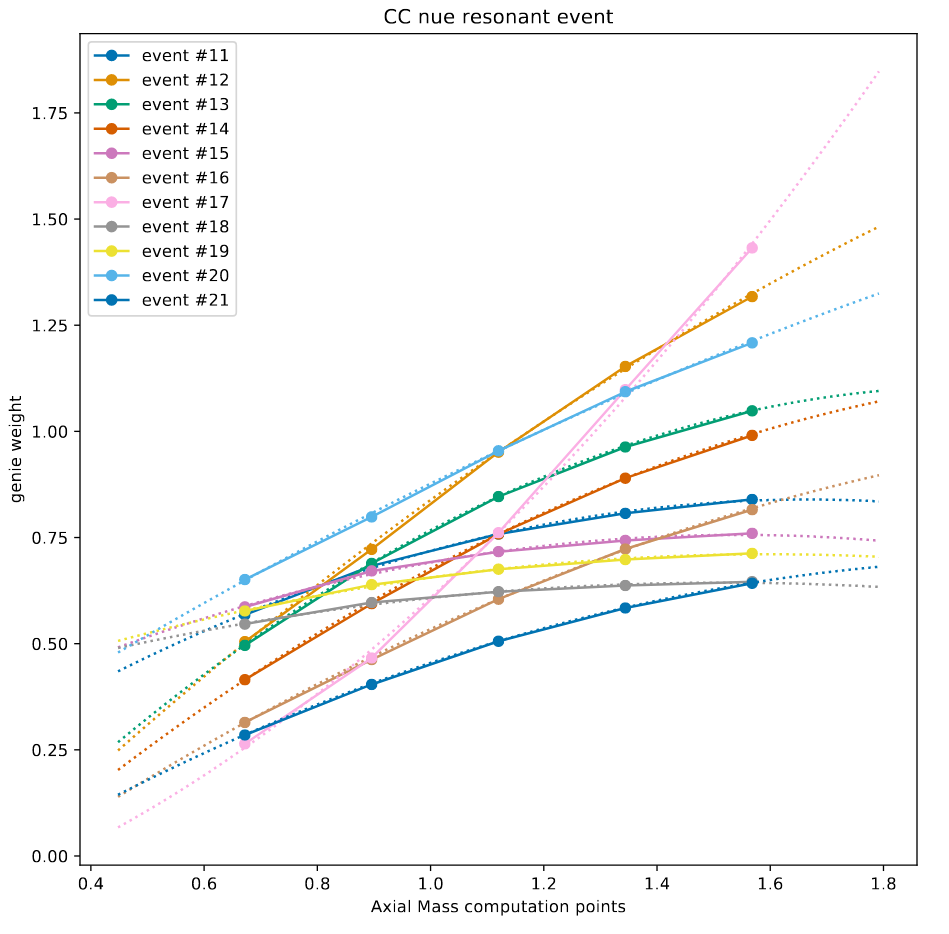
\includegraphics[width=0.5\textwidth]{figures/measurement/systematics/xsec/nue_cc_res_xsec_Ma_systematic.png}
    \tikzsetnextfilename{genie_sys_res}%
\begin{tikzpicture}

%% List of nue CC RES  events

\begin{axis}[
        xlabel=$\Delta M_{\mathrm{A}}^{\mathrm{CCRES}} / \sigma$,
        ylabel=\textsc{GENIE} weight,
        xmajorgrids, ymajorgrids,
        ymin=0.18, ymax=1.58,
        height=0.6\linewidth,
        width=0.8\linewidth,
        legend columns=2,
        legend style={mark=*, at={(0.05,0.95)}, anchor=north west}
    ]
\addplot[orange, domain=-2.2:2.2] {0.3504939715034138 * (1 + 0.11131609002187497 * x + -0.022932572545202236 * x^2};
\addlegendentry{event \#1}
\addplot[orange, only marks, forget plot] coordinates {
(-2, 0.2390467380668949)
(-1, 0.3066640473685763)
(0, 0.3504939715034138)
(1, 0.378941696047475)
(2, 0.397986006147438)
};

\addplot[skyblue, domain=-2.2:2.2] {0.7582274008087017 * (1 + 0.051334614671670824 * x + -0.013918323402408417 * x^2};
\addlegendentry{event \#2}
\addplot[skyblue, only marks, forget plot] coordinates {
(-2, 0.6361056338725656)
(-1, 0.716261703894783)
(0, 0.7582274008087017)
(1, 0.7824732034456762)
(2, 0.7976164413672049)
};

\addplot[bluishgreen, domain=-2.2:2.2] {0.8814816065644564 * (1 + 0.03273351968623338 * x + -0.009338762415529337 * x^2};
\addlegendentry{event \#3}
\addplot[bluishgreen, only marks, forget plot] coordinates {
(-2, 0.789189629008826)
(-1, 0.8507716696219192)
(0, 0.8814816065644564)
(1, 0.8987912601423985)
(2, 0.9094498113562377)
};

\addplot[yellow, domain=-2.2:2.2] {0.9483635232904346 * (1 + 0.26999687193847616 * x + 0.00565034846932953 * x^2};
\addlegendentry{event \#4}
\addplot[yellow, only marks, forget plot] coordinates {
(-2, 0.4643360012427789)
(-1, 0.6781015441978948)
(0, 0.9483635232904346)
(1, 1.2230743122646268)
(2, 1.4721255409542606)
};

\addplot[blue, domain=-2.2:2.2] {0.6341971566788007 * (1 + 0.22525771528791444 * x + -0.019807510312081195 * x^2};
\addlegendentry{event \#5}
\addplot[blue, only marks, forget plot] coordinates {
(-2, 0.29866260486349816)
(-1, 0.47226711305160485)
(0, 0.6341971566788007)
(1, 0.7653501328716419)
(2, 0.8664101077312704)
};

\end{axis}

\end{tikzpicture}

    \caption{\textsc{GENIE} interaction weights as a function of the pull of the axial mass term $M_{A}^{\mathrm{CCRES}}$, for five $\nu_{e}$ CC events produced via resonance interactions. Each dot represents a discrete point for which the event's cross section is computed in \textsc{GENIE}. The  line represents the quadratic fit made used to interpolate the weight value over the continuous range allowed for the systematic parameter.}
    \label{fig:resonant_mass}
\end{figure}

\begin{figure}[!t] 
    \centering
    \begin{subfigure}[t]{0.9\textwidth}
        \centering
        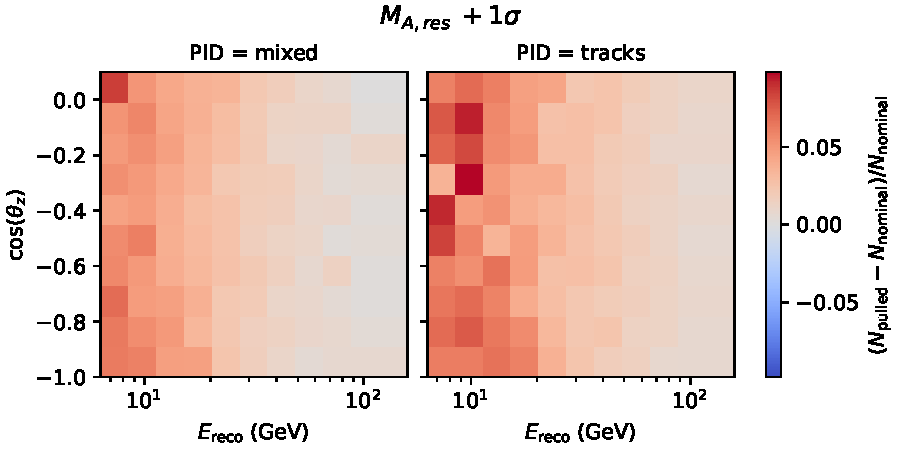
\includegraphics[width=0.99\textwidth,trim={0 0 0 0.6cm},clip]{figures/measurement/systematics/xsec/Genie_Ma_RES.pdf}
        \caption{GENIE $M_{A}^\mathrm{RES}$}
    \end{subfigure}
    \begin{subfigure}[t]{0.9\textwidth}
        \centering
        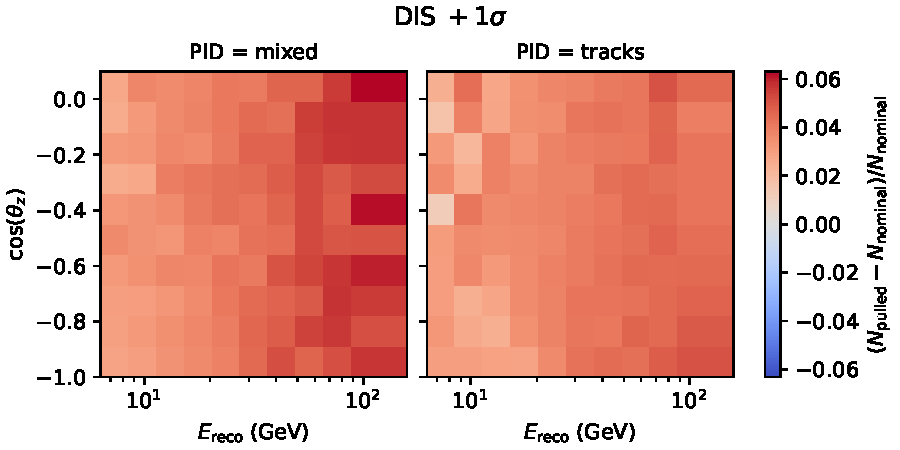
\includegraphics[width=0.99\textwidth,trim={0 0 0 0.6cm},clip]{figures/measurement/systematics/xsec/dis_csms.pdf}
        \caption{DIS CSMS}
    \end{subfigure}  
  \caption{Fractional difference in event rates between (top )$M_{A}^\mathrm{RES}$ (bottom) dis$\_$csms at 1$\sigma$ and at nominal value for both PID bins.
  \label{fig:template_xsecsyst}}
\end{figure}

The uncertainty on the DIS cross-section is primarily given by the disagreement in DIS calculation between CSMS and GENIE cross-sections at energies above 100~GeV. This analysis includes a parameter that interpolates between these two calculations with a linear extrapolation to energies below 100~GeV.
The bottom panel of figure~\ref{fig:template_xsecsyst} illustrates an example of the varying this parameter, DIS, on the final level sample. As expected, the impact of the parameter is largest in the highest energy bins.

There is an additional uncertainty of 20\% on the normalization of NC events to account for uncertainties of the hadronization process and the Weinberg angle.

\subsection{Atmospheric muons}
As events propagate through the offline filter steps described in section~\ref{sec:offline-filter}, the rate of atmospheric muons decreases by several orders of magnitude. This makes it challenging to produce a sufficiently large amount of simulated muon events to accurately estimate the expected background at the final level. To overcome this challenge, two separate muon simulation sets are produced, one of which is used to tune the lower level (up to L4) offline filters and the other is used to estimate muon background at levels L5 and above. 

For both sets, atmospheric muons are generated on the surface of a cylinder encompassing the entire IceCube detector with a radius of 800~m and a height of 1600~m. Positions and directions are sampled according to a flux expectation derived from cosmic ray flux model described in \sidecite{Gaisser:2011klf} and the \textsc{SIBYLL 2.1}\sidecite{sibyll} hadronic interaction model, the same flux model that is also used to weight the simulated events. For the simulations used to tune the lower selection levels, the muon energy is sampled from a power law with a spectral index of -3 and all events are accepted to cover the entire IceCube array. To produce the simulation that is used starting at the L5 trigger level, muons are only accepted if they intersect an inner cylinder centered in the DeepCore fiducial volume with a radius of 180~m and a height of 400~m. Furthermore, muons are rejected based on a KDE estimate of the muon density in energy and zenith angle at the L5 filter level. In this way, the sampling preferably produces such muon events that have a higher chance of passing the offline filtering up to L5, which greatly improves the efficiency of the simulation production.

After the position, direction and energy for a muon has been sampled, its propagation and photon production is simulated using \textsc{PROPOSAL} in just the same way as any muon that is produced in neutrino interaction would be.


\subsection{Photon Propagation}
\label{sec:photon-propagation}

Photons are individually traced through the ice using the GPU-accelerated \textsc{clsim}\cite{clsim} package, which is an \textsc{OpenCL} re-implementation of the Photon-Propagation Code\sidecite{ppc}.  The ice is modeled as 10~m thick layers with individual scattering and absorption lengths that are shown in Figure~\ref{fig:spice-model}. The ice model used for the simulation in this work also incorporates the fact that the ice layers are slightly tilted with respect to the vertical axis, and that scattering and absorption distances are not uniform as a function of azimuth. For every photon, \textsc{clsim} first samples the absorption length from an exponential distribution where the expectation value is the absorption length of the current layer. It then propagates all photons in parallel steps, where every step corresponds to one scattering event and the step length is sampled from an exponential distribution where the expectation value is the scattering length of the current layer. The scattering angle is then sampled from a mixture of a Henyey-Greenstein distribution and a simplified Mie scattering distribution, where the shape parameters of these distributions have previously been calibrated using the in-situ LED calibration system\sidecite{flasher_calibration}. The algorithm determines after every step if the photon has either reached its total absorption length or if it has intersected a DOM and stops its propagation if that is the case. After all photons have either been absorbed or reached a sensor, the simulations stops and passes the photons that reached a sensor on to the next step simulating the detector response.

\begin{figure}
    \centering
    %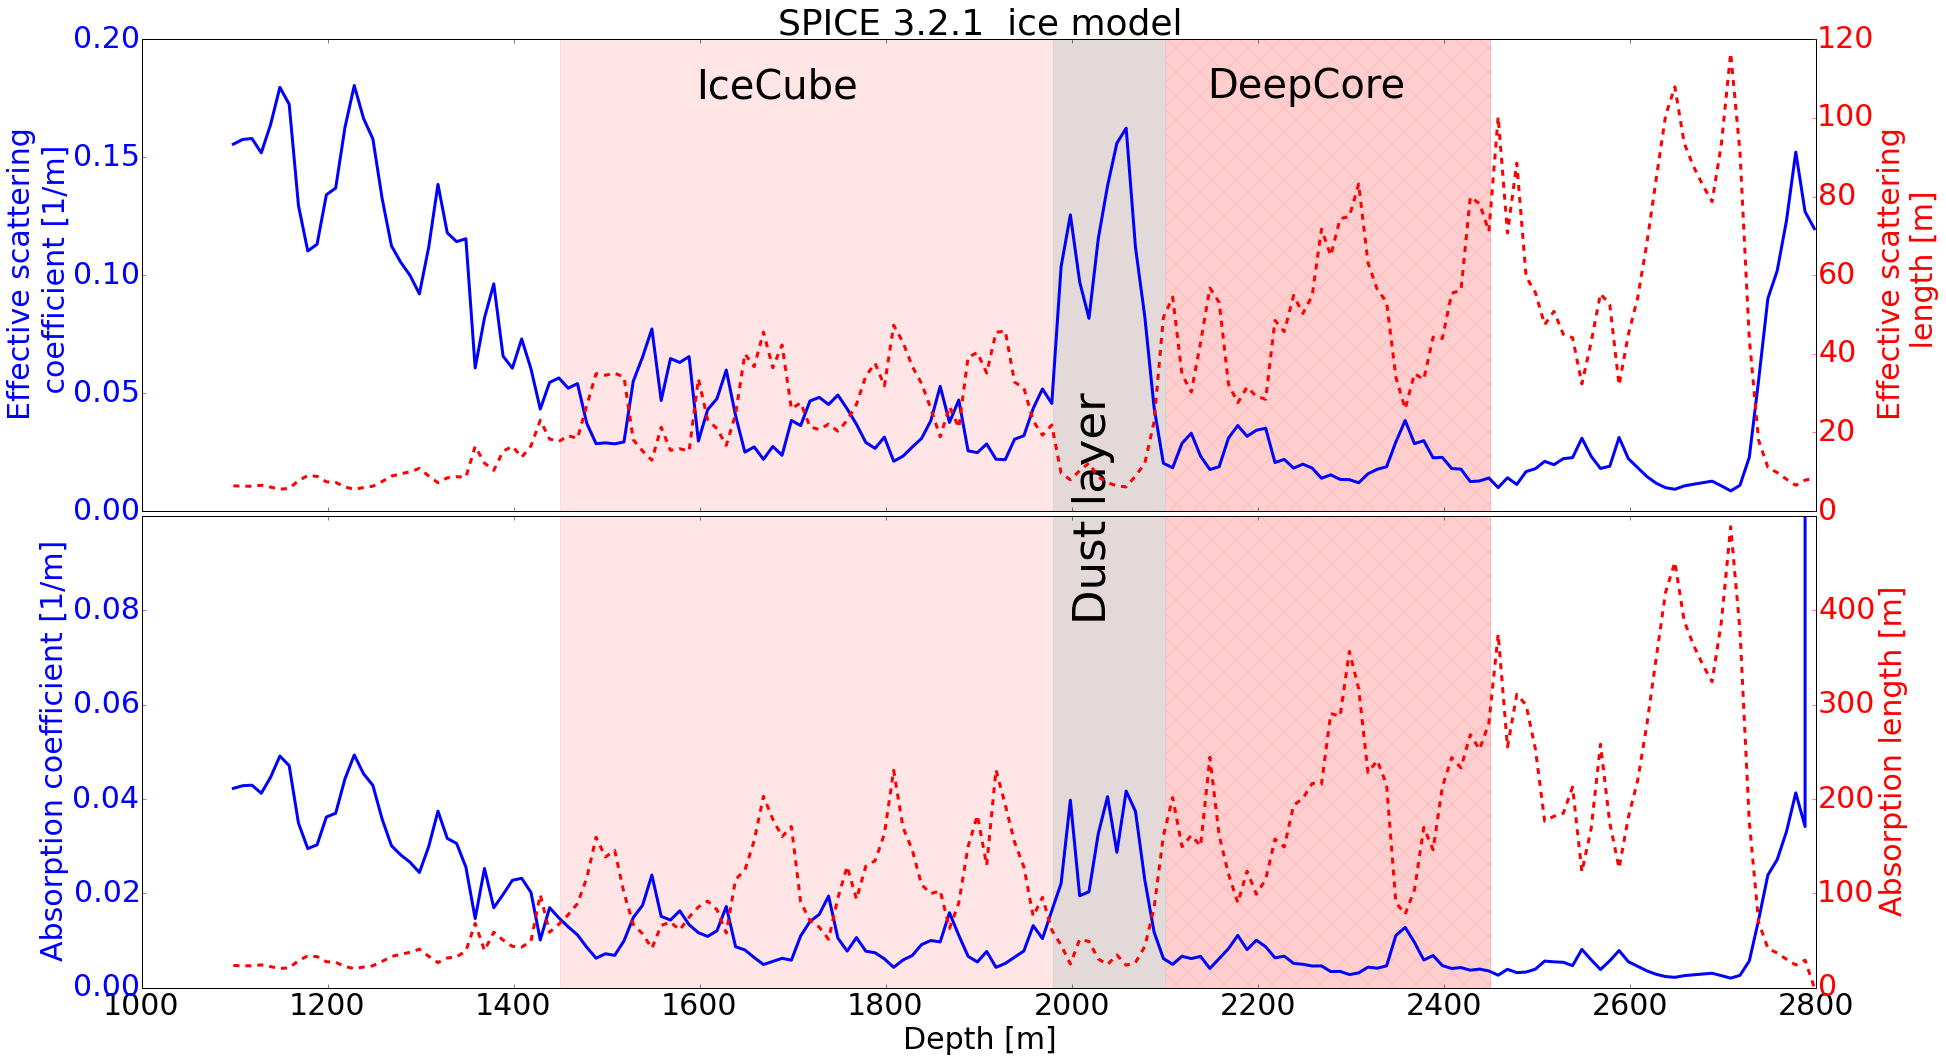
\includegraphics[width=0.9\linewidth]{figures/icecube/ice/Spice3.2.1_layered_scatt_abs_withlength_annotated.png}
    \tikzsetnextfilename{spice_model}%
\begin{tikzpicture}
% let both axes use the same layers
\pgfplotsset{set layers}

\pgfplotstableread{figures/icecube/ice/spice_model/spice_3.2.1/icemodel.dat}\table

\begin{axis}[
    scale only axis,
    width=0.7\linewidth,
    height=0.5\linewidth,
    xmin=1100,xmax=2900,
    xticklabel style={/pgf/number format/.cd,1000 sep={}},
    axis y line*=left, % the '*' avoids arrow heads
    ymin=0,
    enlarge y limits=true,
    xlabel=depth (m),
    ylabel=Scattering length (m),
]
    \addplot[black, thick] table [x index=0, y expr=1 / \thisrowno{1}] \table;
    
    % dust layer
    \draw [name path=dust layer top, gray, thin] (2000, \pgfkeysvalueof{/pgfplots/ymin}) -- (2000, \pgfkeysvalueof{/pgfplots/ymax}); 
    \draw [name path=dust layer bottom, gray, thin] (2100, \pgfkeysvalueof{/pgfplots/ymin}) -- node[near end, sloped, above, black, font=\footnotesize\sffamily] {dust layer} (2100, \pgfkeysvalueof{/pgfplots/ymax});
    \addplot [gray, opacity=0.4] fill between [of=dust layer top and dust layer bottom];
    
    % IceCube
    \draw [name path=icecube top, gray, thin] (1450, \pgfkeysvalueof{/pgfplots/ymin}) -- (1450, \pgfkeysvalueof{/pgfplots/ymax}); 
    \draw [name path=icecube bottom, gray, thin] (2000, \pgfkeysvalueof{/pgfplots/ymin}) -- (2000, \pgfkeysvalueof{/pgfplots/ymax});
    \node[anchor=south, black, font=\footnotesize\sffamily] at (1750, 110) {IceCube\strut};
    \addplot [gray, opacity=0.2] fill between [of=icecube top and icecube bottom];
    
    % DeepCore
    \draw [name path=deepcore top, gray, thin] (2100, \pgfkeysvalueof{/pgfplots/ymin}) -- (2100, \pgfkeysvalueof{/pgfplots/ymax}); 
    \draw [name path=deepcore bottom, gray, thin] (2450, \pgfkeysvalueof{/pgfplots/ymin}) -- (2450, \pgfkeysvalueof{/pgfplots/ymax});
    \node[anchor=south, black, font=\footnotesize\sffamily] at (2270, 110) {DeepCore\strut};
    \addplot [gray, opacity=0.1] fill between [of=deepcore top and deepcore bottom];
    
\end{axis}

\begin{axis}[
    orange,
    scale only axis,
    width=0.7\linewidth,
    height=0.5\linewidth,
    xmin=1100,xmax=2900,
    axis y line*=right,
    axis x line=none,
    ymin=0,
    enlarge y limits=true,
    ylabel=Absorption length (m),
]
    \addplot[orange, thick] table [x index=0, y expr=1 / \thisrowno{2}] \table;

\end{axis}

\end{tikzpicture}

    \caption{Scattering and absorption lengths as a function of depth in the South Pole Ice (SPICE) model that is used to produce the simulation for this work.}
    \label{fig:spice-model}
\end{figure}


\subsection{Simulation of Detector Response}

After the photons have reached the surface of the optical sensors, the simulation determines for each one if it is converted into a Monte-Carlo photo-electron (MCPE). The probability that this occurs depends on the wavelength-dependent sensitivity of the DOM, as well as the angular acceptance. The angular acceptance not only depends on the geometry of the DOM itself, but also incorporates the effect of the re-frozen column of ice surrounding each string. If a photon is accepted and converted into an MCPE, the next step is to simulate how much charge would be measured by the PMT inside the DOM as a response. The charge is drawn from a combination of a normal distribution and two exponential distributions whose parameters have been calibrated \emph{in-situ} to match the observed charge distribution in each individual DOM\sidecite{ic_spe_20}. This distribution, also referred to as the Single Photo-Electron (SPE) template, is shown in Figure~\ref{fig:spe-templates}. The MCPEs with the samples charge are then converted into simulated waveforms for the ATWD and fADC readouts which are then passed into the data processing chain starting from the \emph{wavedeform} algorithm described in Section~\ref{sec:dom-daq}. From there, the simulated events pass through all the same trigger and filter steps that are described in Section~\ref{sec:data-processing}.

\begin{figure}
    \centering
    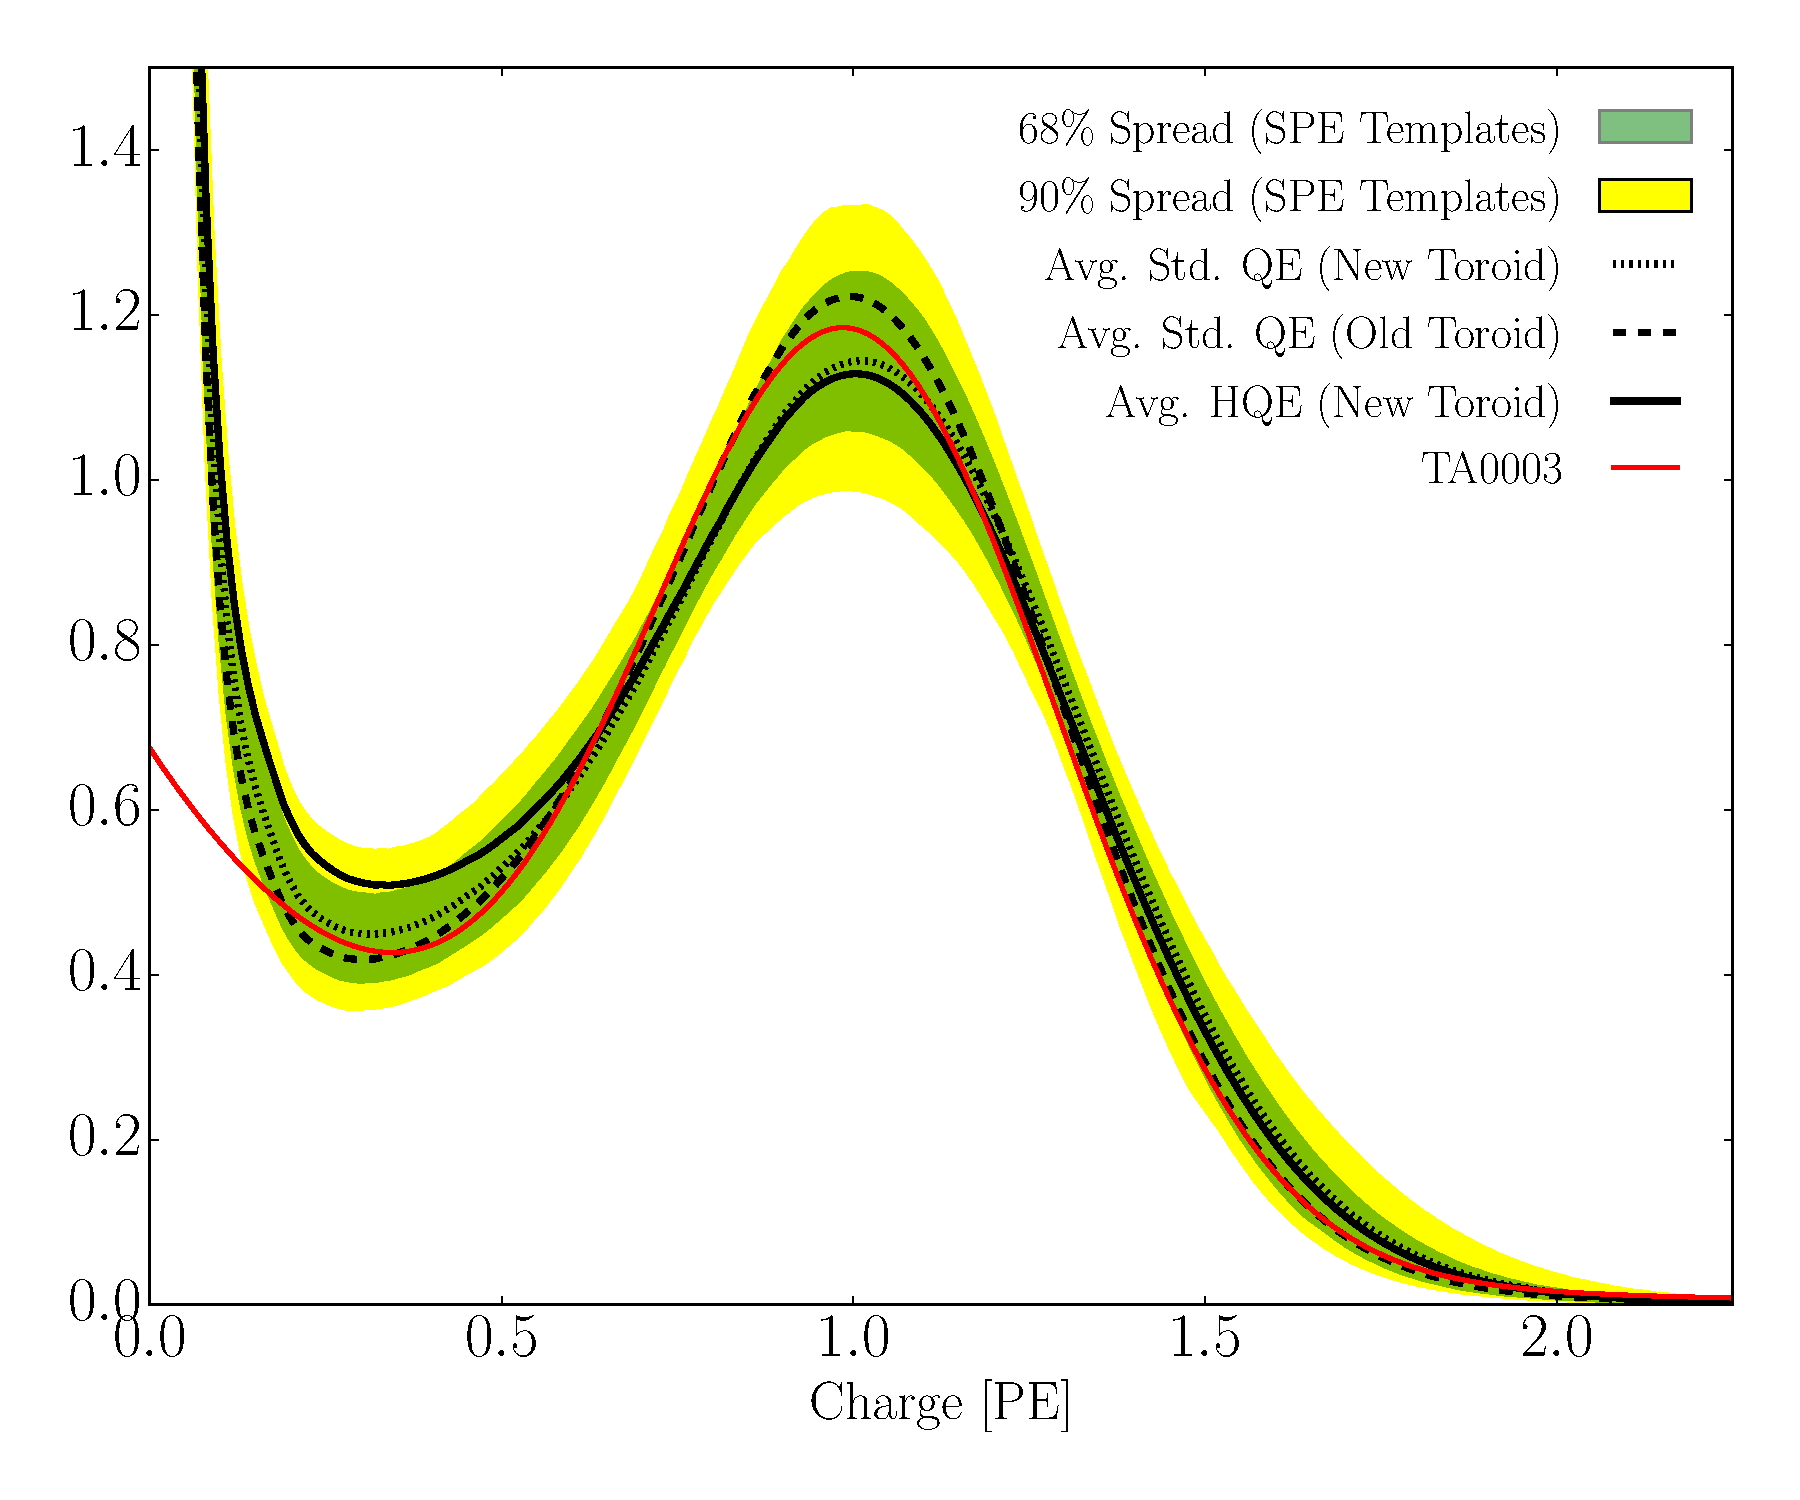
\includegraphics[width=0.8\linewidth]{figures/icecube/detector_response/SPE_TA003_2.pdf}
    \caption{The green (yellow) regions show the 68\% (90\%) spread in the SPE charge templates for a given charge.  Superimposed are the average SPE charge templates for the variety of hardware configurations shown in the black dotted, dashed, and solid lines. The TA0003 distribution, shown in red, originates from laboratory measurements. Figure taken from \cite{ic_spe_20}.}
    \label{fig:spe-templates}
\end{figure}

\subsubsection{Detector Noise}

\begin{margintable}
\caption{\label{tab:vuvuzela_params} Parameters used in the noise simulation. }
    \begin{tabular}{lc}\toprule
        \textbf{Parameter} & \textbf{Unit} \\ \midrule
        Thermal rate &  $s^{-1}$ \\ 
        Decay rate &  $s^{-1}$ \\
        Decay hits &  hits \\ 
        Decay hits mean &  $\log_{10} (ns) $\\ 
        Decay hits sigma &  $\log_{10} (ns) $ \\ \bottomrule
    \end{tabular}
\end{margintable}
Detector noise in IceCube consists mostly of photons produced in radioactive decay inside the glass housing of the DOMs and the PMTs. However, the simulation does not simulate the propagation of these photons. Instead, noise MCPEs are directly sampled from distributions that take both thermal and non-thermal noise components into account.The thermal component comes from uncorrelated photons and PMT dark noise and is modeled as a Poisson process with a constant rate. The non-thermal component comes from correlated bursts of photons that are produced by radioactive decays. To simulate it, decay times are first drawn from a Poisson process with a constant rate, and the number of photons produced in each decay is sampled from a Poisson distribution. The time differences between the non-thermal MCPEs produced by each decay are then sampled from a Log-Gaussian distribution. This simulation method has five free parameters listed in Table~\ref{tab:vuvuzela_params} that are calibrated \emph{in-situ} for every DOM. All thermal and non-thermal MCPEs are injected into each simulated event together with the MCPEs from photons and passed into the rest of the simulation chain.
% \begin{margintable}
% \caption{\label{tab:vuvuzela_params} Parameters used in the noise simulation. }
%     \begin{tabular}{lcc}\toprule
%         \textbf{Parameter} & \textbf{Designation} & \textbf{Unit} \\ \midrule
%         Thermal rate & $\lambda_{Th}$ & $s^{-1}$ \\ 
%         Decay rate & $\lambda_{Decay}$ & $s^{-1}$ \\
%         Scintillation hits & $\eta_{Scint}$ & hits \\ 
%         Scintillation mean & $\mu_{Scint}$ & $\log_{10} (ns) $\\ 
%         Scintillation sigma & $\sigma_{Scint}$ &  $\log_{10} (ns) $ \\ \bottomrule
%     \end{tabular}
% \end{margintable}

\subsection{Variation of Detector Properties}
\label{sec:detector-unc}
Systematic uncertainties on the detector properties that need to be taken into account are the overall optical efficiency of the DOMs as well as the properties of the surrounding ice. The parametrization and priors of each of these properties are informed by IceCube calibration studies. 
\begin{itemize}
    \item DOM efficiency: A factor that scales the probability that a photon hitting the PMT of a DOM will produce a photo-electron that is measured by the electronics. Nominal value is 1, prior standard deviation is 10\%.
    \item Hole ice: Two parameters describe the effect of the optical properties of the column of re-frozen ice within the bore holes in which the strings have been deployed. The details of this parametrization is described below.
    \item Bulk ice: The over-all absorption and scattering coefficients of all ice layers are multiplied by a scaling factor. The nominal value for ice absorption is 1.0 with a prior standard deviation of 5\%. The nominal value for ice scattering is 1.05 with a prior standard deviation of 10\%.
\end{itemize}

In total, the uncertainties on the detector properties is modeled by five  parameters, one for the DOM efficiency, two for the hole ice model and two for the bulk ice uncertainty. To model the effect of these parameters on the analysis histogram, several MC sets at different variations of DOM efficiency, hole ice, and bulk ice parameters are produced. These MC sets are used to find a parametrization that will model how the distribution of events in energy, zenith and PID will change as a function of these parameters.

\subsubsection{Hole Ice Parametrization}
\label{sec:hole-ice-parametrization}

The bore holes in which IceCube's strings have been deployed were drilled using hot water to melt a column of ice into which the strings with their attached optical sensors could be lowered. This water column re-froze after deployment to form what is referred to as \emph{hole ice}\sidecite{Fiedlschuster:2019unl}. Camera observations of this re-freezing process suggest that the hole ice is transparent near the edges of be hole and contains a bubble column in its center\sidecite{rongen2016measuring}. This is consistent with the expectation of the re-freezing process, where bubbles and impurities are pushed towards the center as the outer edges begin to freeze. The bubble column has a much shorter scattering length than the surrounding bulk ice and therefore decreases the probability of a photon entering a DOM directly from below.
The effect of the re-frozen ice column surrounding the strings can be modeled as a modification to the optical efficiency of the DOMs as a function of the incident angle of incoming photons. In the past, many different angular acceptance curves have been produced from \emph{in-situ} calibration measurements as well as the best fit results of previous DeepCore oscillation analyses, in addition to the laboratory measurements that have been made in water tanks before the deployment of IceCube. For the analysis presented in this work, a two-dimensional parametrization was developed that can approximate any of these hole ice models such that it can be used as a \emph{unified} hole ice model. To do this, all previous angular acceptance curves are evaluated as a function of the cosine of the photon incidence angle, $\cos(\eta)$, at 100 points over the entire valid domain between -1 and 1, where 1 represents a photon entering a DOM directly from below. Using Principal Component Analysis, the variations between the different models are decomposed into a mean and the most important components that explain the variance between models. It was found that the two most important components, $p_0$ and $p_1$, describe all known hole ice models adequately. Their effect is shown in \reffig{hole-ice-parametrization} as variations with the acceptance curve that is used as the baseline in this analysis. The right panel of \reffig{hole-ice-parametrization} also shows where the older hole ice models are located in the space spanned by $p_0$ and $p_1$. The laboratory measurement, which did not include any hole ice effects, notably lies far outside of the region of all other hole ice models that are all produced \emph{in-situ}.

\begin{figure*}
    \centering
    \tikzsetnextfilename{hole_ice_p0_p1}%
\begin{tikzpicture}

\pgfplotstableread{figures/measurement/systematics/detector/hole_ice/angsens_example_fluct.csv}\table
\pgfplotstableread{figures/measurement/systematics/detector/hole_ice/all_acceptance_curves.csv}\acceptancecurves

\begin{axis}[
        width=0.45\linewidth, height=0.4\linewidth,
		xmajorgrids, ymajorgrids,
		xlabel=$\cos(\eta)$, ylabel=relative optical efficiency,
		legend style={at={(0.02,0.95)}, anchor=north west},
        ytick distance=0.2,
	]
    \addplot[black, thick] table [x=cos_theta, y=baseline] \acceptancecurves;
    \addlegendentry{baseline}
    
    \addplot[vermilion, thick] table [x=cos_theta, y=nominal] \acceptancecurves;
    \addlegendentry{laboratory}
    
    % \addplot[bluishgreen, thick] table [x=cos_theta, y=bfp_three_flav] \acceptancecurves;
    % \addlegendentry{best fit}
    
    \addplot[blue, thin, name path=fluct_p0_dn, forget plot] table [x=cos_theta, y=fluct_p0_dn] \table;
    \addplot[blue, thin, name path=fluct_p0_up, forget plot] table [x=cos_theta, y=fluct_p0_up] \table;
    \addplot[blue, opacity=0.5] fill between[of = fluct_p0_dn and fluct_p0_up];
    \addlegendentry{example variation in $p_0$}
    
    \addplot[orange, thin, name path=fluct_p1_dn, forget plot] table [x=cos_theta, y=fluct_p1_dn] \table;
    \addplot[orange, thin, name path=fluct_p1_up, forget plot] table [x=cos_theta, y=fluct_p1_up] \table;
    \addplot[orange, opacity=0.5] fill between[of = fluct_p1_dn and fluct_p1_up];
    \addlegendentry{example variation in $p_1$}
	
\end{axis}
\end{tikzpicture}
    \tikzsetnextfilename{hole_ice_models_scatter}%
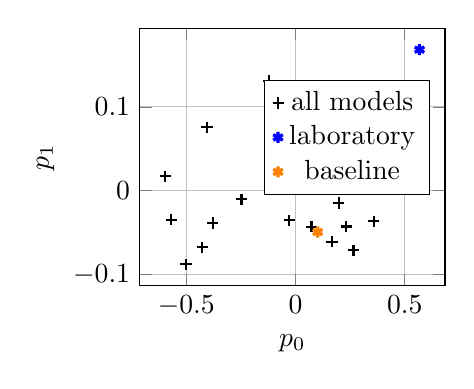
\begin{tikzpicture}
\begin{axis}[
        width=0.45\linewidth, height=0.4\linewidth,
		xmajorgrids, ymajorgrids,
		xlabel=$p_0$,
		ylabel=$p_1$,
		legend columns=1,
		legend style={
			/tikz/every even column/.append style={column sep=0.2cm},
			at={(0.95, 0.8)},
			anchor=north east
		}
        % ytick={-0.1, -0.05, 0, 0.05, 0.1},
        % yticklabels={-0.1, -0.05, 0, 0.05, 0.1}
	]
    \addplot[black, only marks, mark=+, thick] table [x=p0, y=p1] {
       	name	p0	p1
        %nominal	0.567771	0.168269
        h1-100cm	-0.123027	0.131104
        h2-50cm	-0.405128	0.075841
        h3-30cm	-0.595997	0.017468
        dima	0.232258	-0.042754
        dima+	0.265798	-0.070837
        dima-	0.198792	-0.014733
        dragon	0.072961	-0.043175
        greco	0.167150	-0.060809
        %baseline	0.101569	-0.049344
        msu2	0.357705	-0.036428
        martin-0.6-14	-0.028113	-0.035254
        martin-0.8-40	-0.246929	-0.010401
        martin-1.8-125	-0.569511	-0.034839
        all	-0.427318	-0.067581
        tilted	-0.501349	-0.087664
        horizontal	-0.378935	-0.038564
    };
    \addlegendentry{all models}
    \addplot[blue, only marks, mark=asterisk, very thick] coordinates {
        (0.567771,	0.168269)
    };
    \addlegendentry{laboratory}
    \addplot[orange, only marks, mark=asterisk, very thick] coordinates {
        (0.101569,	-0.049344)
    };
    \addlegendentry{baseline}
    

	
\end{axis}
\end{tikzpicture}
    \caption{Two parameter model used to parametrize the optical efficiency in this analysis (left) and the positions in this two-dimensional space where older hole ice models are located (right).}
    \label{fig:hole-ice-parametrization}
\end{figure*}

\subsubsection{Depth-dependent ice properties}
\label{sec:depth-dependent-ice-properties}

In the parametrization of the uncertainties of the detector properties described in \refsec{detector-unc}, variations of the scattering and absorption coefficients are only described by global, depth-independent scaling factors. In principle, the error on the properties of the ice could also change as a function of depth. Of particular interest for the analysis presented in this work are variations of the ice properties at length scales of the DeepCore fiducial volume located within DeepCore. Variations at much longer scales would be indistinguishable from uniform variations given the size of the event signatures observed below 100~GeV, while variations at much shorter scales are expected to average out. To test how significantly such a variation would impact the final level histograms, two MC sets are produced in which the scattering and absorption coefficients vary following a sigmoid function function centered in DeepCore with an amplitude of $\pm 2\%$ in opposing directions as shown in \reffig{step-function-ice-model}.
\begin{figure}
    \centering
    %\missingfigure[figwidth=0.8\linewidth]{Show step function variations, see  \href{https://drive.google.com/file/d/1TV0r1VzRbRPxlQeeCuq8DaZzeQloJZ_J/view}{presentation on lowen call}.}
    \tikzsetnextfilename{ice_step_func_perturbations}%
\begin{tikzpicture}
\begin{axis}[
    height=0.5\linewidth,
    width=0.8\linewidth,
    xmin=1100,xmax=2900,
    xticklabel style={/pgf/number format/.cd,1000 sep={}},
    ymin=0.97, ymax=1.03,
    enlarge y limits=true,
    xlabel=depth (m),
    legend columns=2,
    ylabel=perturbation factor,
    xmajorgrids, ymajorgrids
]
    \addplot[black, thick] table [x=depth, y=perturbation1, col sep=comma] {figures/measurement/systematics/detector/ice_perturbation/ice_perturbations.csv};
    \addlegendentry{perturbation +2\%}
    
    \addplot[orange, thick] table [x=depth, y=perturbation2, col sep=comma] {figures/measurement/systematics/detector/ice_perturbation/ice_perturbations.csv};
    \addlegendentry{perturbation -2\%}
    % dust layer
    \draw [name path=dust layer top, gray, thin] (2000, \pgfkeysvalueof{/pgfplots/ymin}) -- (2000, \pgfkeysvalueof{/pgfplots/ymax}); 
    \draw [name path=dust layer bottom, gray, thin] (2100, \pgfkeysvalueof{/pgfplots/ymin}) -- node[sloped, above, black, font=\footnotesize\sffamily] {dust layer} (2100, \pgfkeysvalueof{/pgfplots/ymax});
    \addplot [gray, opacity=0.4] fill between [of=dust layer top and dust layer bottom];
    
    % IceCube
    \draw [name path=icecube top, gray, thin] (1450, \pgfkeysvalueof{/pgfplots/ymin}) -- (1450, \pgfkeysvalueof{/pgfplots/ymax}); 
    \draw [name path=icecube bottom, gray, thin] (2000, \pgfkeysvalueof{/pgfplots/ymin}) -- (2000, \pgfkeysvalueof{/pgfplots/ymax});
    \node[anchor=south, black, font=\footnotesize\sffamily] at (1750, 0.97) {IceCube\strut};
    \addplot [gray, opacity=0.2] fill between [of=icecube top and icecube bottom];
    
    % DeepCore
    \draw [name path=deepcore top, gray, thin] (2100, \pgfkeysvalueof{/pgfplots/ymin}) -- (2100, \pgfkeysvalueof{/pgfplots/ymax}); 
    \draw [name path=deepcore bottom, gray, thin] (2450, \pgfkeysvalueof{/pgfplots/ymin}) -- (2450, \pgfkeysvalueof{/pgfplots/ymax});
    \node[anchor=south, black, font=\footnotesize\sffamily] at (2270, 0.97) {DeepCore\strut};
    \addplot [gray, opacity=0.1] fill between [of=deepcore top and deepcore bottom];
    
\end{axis}

\end{tikzpicture}

    \caption{Perturbation of the scattering and absorption coefficients with respect to the nominal ice model applied in additional MC sets.}
    \label{fig:step-function-ice-model}
\end{figure}
The size of this variation corresponds approximately a $1\sigma$-allowed variation according to flasher calibration data. For every bin in the final analysis histogram, a linear regression is fit to the bin counts of the nominal MC set and the two variations. By comparing the $\chi^2$ test statistic resulting from the regression with the free fit and a regression where the slope is fixed to zero, a p-value can be calculated for every bin, where the null hypothesis is that the step-function variation has no effect. The p-values for all analysis bins are shown in \reffig{steppiness-pvals} and are consistent with random fluctuations. Therefore, it was concluded that the effect of a depth-dependent ice model variation is well within the statistical uncertainty of the simulation and need not be included in the measurement.
\begin{figure}
    \centering
    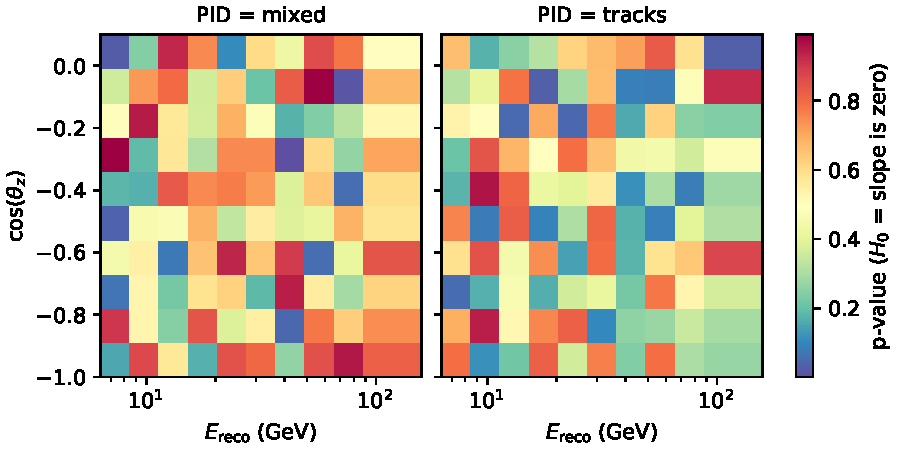
\includegraphics[width=\linewidth]{figures/measurement/systematics/detector/ice_perturbation/steppiness_slope_pvals_verification_sample.pdf}
    \caption{Bin-wise p-value of the fitted slopes as a function of the step-function ice model variation.}
    \label{fig:steppiness-pvals}
\end{figure}

\subsection{Variation of the Atmospheric Neutrino Flux}
\label{sec:flux_systs}

The atmospheric neutrino flux can vary depending on the choice of primary cosmic ray (CR) model, assumed meson yield, hadronic interaction (HI) model and atmospheric density model that are used in the calculation. The nominal flux, $\Phi_\mathrm{nom}$, is modified to a systematic flux, $\Phi_\mathrm{sys}$, so that

\begin{equation}
    \Phi_{\mathrm{sys}}(E) = \Phi_{\mathrm{nom}} \cdot \left( \frac{E}{E_\mathrm{pivot}}\right)^{\Delta \gamma}
    +
    \sum_{i=1}^{N_\mathrm{Barr}} B_i \cdot \frac{\mathrm{d} \Phi_{\mathrm{nom}}}{\mathrm{d}B_i}\label{eq:flux-variation}
\end{equation}

The first term in \refeq{flux-variation} is due to the CR flux uncertainty and corresponds to shifting the spectral index of the neutrino flux, with a pivot point at $E_\mathrm{pivot}=24\;\mathrm{GeV}$. The second term describes the uncertainty of the Pion and Kaon production yield, where each $B_i$ corresponds to the variation in one \emph{Barr block} (further described below). The gradients with respect to these variations, $\frac{\mathrm{d} \Phi_{\mathrm{nom}}}{\mathrm{d}B_i}$, are calculated using the \textsc{MCEq}\cite{mceq, fedynitch2012influence,fedynitch2015calculation} flux calculator.

\subsubsection{Uncertainty on Meson Production}
\labsec{barr-scheme}
The Barr scheme\sidecite{Barr2006} entails dividing the phase space of incident parent particle $E_\mathrm{i}$ and the outgoing secondary particle $E_\mathrm{s}$ (or, equivalently, $x_{\mathrm{LAB}}=E_\mathrm{s}/E_\mathrm{i}$) into regions that are each denoted by a Barr variable. There are eight regions/variables that define the uncertainty on $ \pi^+ $ production, and four regions that define the $K^+$ production, as shown in \reffig{barr-blocks}. For every region, a different relative uncertainty is assigned based on the experimental constraints in that region, as shown in \reffig{barr-blocks-uncertainty}. For primary particle energies $>500\;\mathrm{GeV}$, an additional energy-dependent term is added to the uncertainty to account for the fact that no accelerator measurements are available at these energies to constrain the meson yield. As the pion ratio is well-measured, the uncertainty on $ \pi^- $ is defined by the uncertainty on $ \pi^+ $ combined with the uncertainty on the pion ratio. The uncertainty on $ K^- $ production is parametrized separately from the $K^+$ production. The only modification to the original Barr scheme used in this analysis is that the low-energy $ \pi^+ $ Barr variables A-F are summarized to a single variable with a relative uncertainty of 63\%, because their impact was found to be highly correlated. Thus the uncertainty from meson production is described by $N_\mathrm{Barr}=17$ Barr variables that enter \refeq{flux-variation}.

\begin{figure}
    \centering
    \tikzsetnextfilename{barr_blocks_annotated}%
\begin{tikzpicture}
    \node[above right, inner sep=0] (image) at (0,0) {
        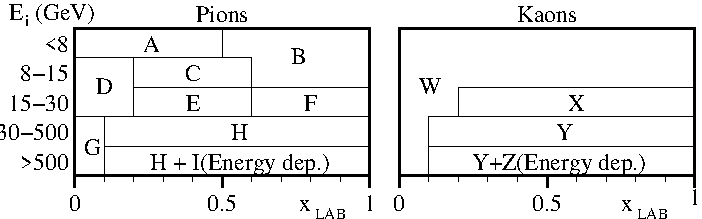
\includegraphics[width=0.8\linewidth]{figures/measurement/systematics/flux/barr_blocks.pdf}
    };
    % Create scope where axes are matching the Pion grid
    \begin{scope}[
        x={($0.42*(image.south east)$)},
        y={($0.67*(image.north west)$)},
        shift={($0.107*(image.south east) + 0.2*(image.north west)$)}
    ]
        % Grid
        %\draw[darkgray,step=0.2] (0,0) grid (1,1);
        \draw[thick, orange, fill=orange, fill opacity=0.8] (0, 0.4) rectangle (1, 1);
        \node[anchor=south, fill=white, draw=black] at (0.5, 0.55) {merged A-F};
    \end{scope}
\end{tikzpicture}
    %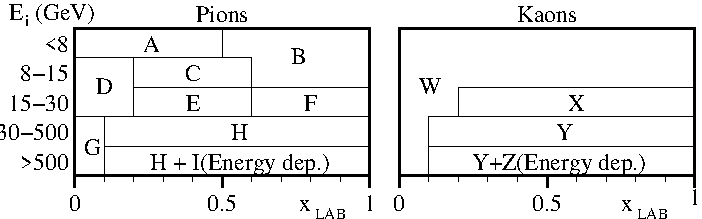
\includegraphics[width=0.8\linewidth]{figures/measurement/systematics/flux/barr_blocks.pdf}
    \caption{Fully correlated regions of uncertainties in the hadronic interaction model. Figure taken from \cite{Barr2006}.}
    \labfig{barr-blocks}
\end{figure}
\begin{figure}
    \centering
    \tikzsetnextfilename{barr_blocks_uncertainty_annotated}%
\begin{tikzpicture}
    \node[above right, inner sep=0] (image) at (0,0) {
        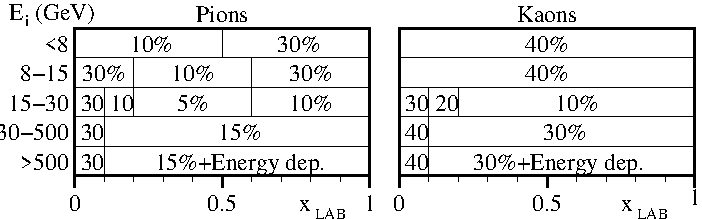
\includegraphics[width=0.8\linewidth]{figures/measurement/systematics/flux/barr_blocks_uncertainty.pdf}
    };
    % Create scope where axes are matching the Pion grid
    \begin{scope}[
        x={($0.42*(image.south east)$)},
        y={($0.67*(image.north west)$)},
        shift={($0.107*(image.south east) + 0.2*(image.north west)$)}
    ]
        % Grid
        %\draw[darkgray,step=0.2] (0,0) grid (1,1);
        \draw[thick, orange, fill=orange, fill opacity=0.8] (0, 0.4) rectangle (1, 1);
        \node[anchor=south, fill=white, draw=black] at (0.5, 0.55) {63\%};
    \end{scope}
\end{tikzpicture}
    %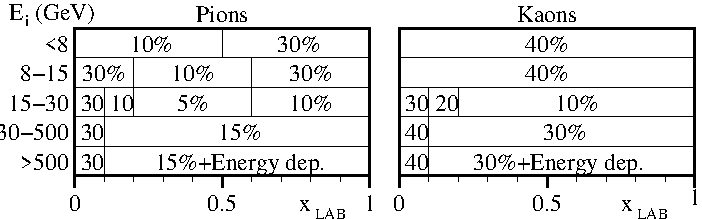
\includegraphics[width=0.8\linewidth]{figures/measurement/systematics/flux/barr_blocks_uncertainty.pdf}
    \caption{Relative uncertainty assigned to each region of hadron phase space in percent. Figure taken from \cite{Barr2006}.}
    \labfig{barr-blocks-uncertainty}
\end{figure}

%Only in the sterile analysis, the prior on the variables with an energy-dependent uncertainty, \texttt{barr\_i\_Pi}, \texttt{barr\_z\_K}, and \texttt{barr\_z\_antiK} by a factor of 5 to 0.61, because it was found that the original priors used in the standard three-flavor analysis greatly under-estimated the impact of these parameters compared to the original Barr 2006 paper.

\subsubsection{Atmospheric density}

The development of particle showers in the atmosphere is governed by competing processes of decay and interactions with the surrounding air. The density of the atmosphere can therefore influence the neutrino production and could potentially contribute a systematic uncertainty to oscillation measurements. The size of the effect of atmospheric density uncertainty on the analysis presented in this work is estimated using the same procedure as described in \cite{MEOWS}. This is done by obtaining a variation of atmospheric density profile by perturbing the Earth’s atmospheric temperature within a prior range given by the NASA Atmospheric InfraRed Sounder (AIRS) satellite~\cite{AIRS} temperature data. The resulting atmospheric density profile are injected into \textsc{MCEq} to calculate new fluxes. This is performed for a variety of CR models and hadronic interaction models available in \textsc{MCEq}. The resulting fluctuations of the neutrino flux observed at the detector were found to be consistently below 1\% for the energy ranges most relevant to DeepCore measurements and is therefore not included as a systematic uncertainty in this work.



